\documentclass[aspectratio=169]{beamer}
\usepackage{fontspec}
\usepackage[vietnamese]{babel}
\usepackage{graphicx}
\usepackage{booktabs}
\usepackage{listings}
\usepackage{caption}

% Cài đặt theme
\usetheme{Madrid}
\usecolortheme{default}
\setbeamertemplate{navigation symbols}{}
\setbeamertemplate{caption}[numbered]
\setbeamertemplate{footline}[frame number]

% Cấu hình listings cho code Python
\lstset{
    language=Python,
    basicstyle=\ttfamily\scriptsize,
    keywordstyle=\color{blue},
    stringstyle=\color{red},
    commentstyle=\color{green!60!black},
    numbers=left,
    numberstyle=\tiny\color{gray},
    stepnumber=1,
    showstringspaces=false,
    tabsize=4,
    breaklines=true,
    breakatwhitespace=true,
    frame=single,
    backgroundcolor=\color{gray!10}
}

\title[Chương 14: CNN trong Computer Vision]{Chương 14: Thị giác Máy tính Chuyên sâu sử dụng Mạng Nơ-ron Tích chập (CNN)}
\author[Giảng viên]{Giảng viên: [Tên Giảng Viên]}
\institute[Đại Học Đông Á]{Đại Học Đông Á}
\date{\today}

\begin{document}

\begin{frame}
    \titlepage
\end{frame}

\begin{frame}{Nội dung Chương 14}
    \tableofcontents
\end{frame}

\section{1. Vỏ Não Thị Giác và Nguồn Gốc CNN}

\begin{frame}{Khởi nguồn của Thị giác Máy tính}
    \begin{itemize}
        \item Năm 1959, David Hubel và Torsten Wiesel thực hiện một thí nghiệm kinh điển trên mèo, phát hiện ra cấu trúc của \textbf{vỏ não thị giác (Visual Cortex)}.
        \item Họ phát hiện rằng các nơ-ron trong vỏ não thị giác có một \textbf{trường tiếp nhận cục bộ (local receptive field)}.
        \item Một số nơ-ron chỉ phản ứng với các đường ngang, một số nơ-ron khác phản ứng với đường dọc hoặc đường chéo.
        \item Các nơ-ron này được sắp xếp theo cấu trúc phân cấp: Nơ-ron cấp thấp nhận diện các đường nét đơn giản, nơ-ron cấp cao kết hợp chúng để nhận diện hình dạng phức tạp hơn.
    \end{itemize}
\end{frame}

\begin{frame}{Trường tiếp nhận cục bộ (Local Receptive Fields)}
    \begin{columns}
        \begin{column}{0.5\textwidth}
            \begin{itemize}
                \item Kiến trúc này đã truyền cảm hứng cho \textbf{Mạng Nơ-ron Tích chập (CNN)}.
                \item \textbf{Hình 14-1} cho thấy thay vì kết nối với mọi pixel (như MLP), mỗi nơ-ron lớp tích chập thứ nhất chỉ kết nối với một vùng hình chữ nhật nhỏ của hình ảnh đầu vào.
                \item Nơ-ron ở lớp thứ hai lại kết nối với một vùng nhỏ của lớp thứ nhất, cứ như vậy tạo ra mạng phân cấp.
            \end{itemize}
        \end{column}
        \begin{column}{0.5\textwidth}
            \centering
            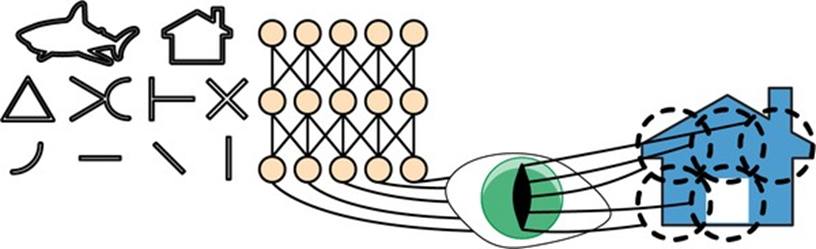
\includegraphics[width=\textwidth,height=0.65\textheight,keepaspectratio]{../machineLearningWeb/Figures/CH14/Hình_14-1}
            \vspace{0.2cm}
            \textit{Hình 14-1: Kiến trúc phân cấp của CNN}
        \end{column}
    \end{columns}
\end{frame}

\section{2. Các thành phần của CNN (Tích chập \& Gộp)}

\begin{frame}{Lớp Tích chập (Convolutional Layer)}
    \begin{columns}
        \begin{column}{0.5\textwidth}
            \begin{itemize}
                \item Lớp Tích chập là khối xây dựng cốt lõi của CNN.
                \item Một nơ-ron ở vị trí $(i, j)$ của một lớp nhất định được kết nối với đầu ra của các nơ-ron ở lớp trước trong vùng từ hàng $i$ đến $i + f_h - 1$, cột $j$ đến $j + f_w - 1$.
                \item \textbf{Hình 14-2} minh họa sự kết nối giữa các lớp.
            \end{itemize}
        \end{column}
        \begin{column}{0.5\textwidth}
            \centering
            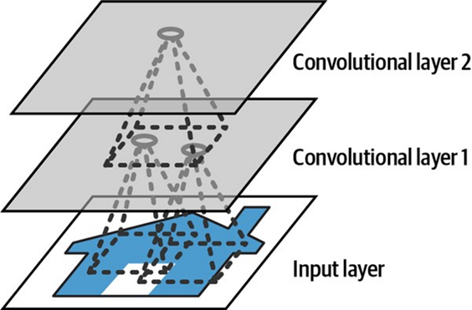
\includegraphics[width=\textwidth,height=0.65\textheight,keepaspectratio]{../machineLearningWeb/Figures/CH14/Hình_14-2}
            \vspace{0.2cm}
            \textit{Hình 14-2: Kết nối cục bộ giữa 2 lớp CNN}
        \end{column}
    \end{columns}
\end{frame}

\begin{frame}{Đệm (Padding)}
    \begin{columns}
        \begin{column}{0.4\textwidth}
            \begin{itemize}
                \item Nếu tiếp tục áp dụng tích chập, ảnh sẽ nhỏ dần đi sau mỗi lớp.
                \item Để giữ nguyên kích thước, ta dùng kĩ thuật \textbf{Zero Padding} (đệm thêm các số 0 xung quanh ảnh).
                \item \textbf{Hình 14-3} (trái): Hình đầu vào 5x5.
                \item \textbf{Hình 14-3} (phải): Hình 5x5 được thêm đệm $p=1$ thành 7x7. Tích chập bằng kernel $3\times3$ sẽ trả về đúng ma trận đầu ra $5\times5$.
            \end{itemize}
        \end{column}
        \begin{column}{0.6\textwidth}
            \centering
            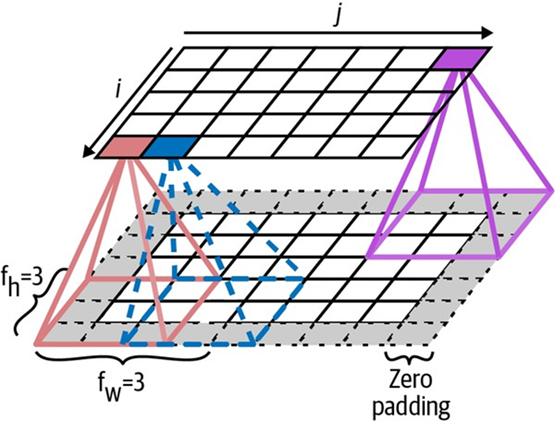
\includegraphics[width=\textwidth,height=0.65\textheight,keepaspectratio]{../machineLearningWeb/Figures/CH14/Hình_14-3}
            \vspace{0.2cm}
            \textit{Hình 14-3: Kết nối với Padding}
        \end{column}
    \end{columns}
\end{frame}

\begin{frame}{Bước nhảy (Strides)}
    \begin{columns}
        \begin{column}{0.5\textwidth}
            \begin{itemize}
                \item Nếu muốn giảm kích thước ảnh đầu ra một cách nhanh chóng, chúng ta sử dụng \textbf{Stride (Bước nhảy) > 1}.
                \item \textbf{Hình 14-4} cho thấy trường tiếp nhận di chuyển $2$ ô mỗi lần ($s=2$).
                \item Kết quả: Một hình ảnh gốc 5x5 áp dụng kernel 3x3 với padding=1 và stride=2 sẽ cho ra bản đồ đặc trưng có kích thước chỉ còn $3\times3$.
            \end{itemize}
        \end{column}
        \begin{column}{0.5\textwidth}
            \centering
            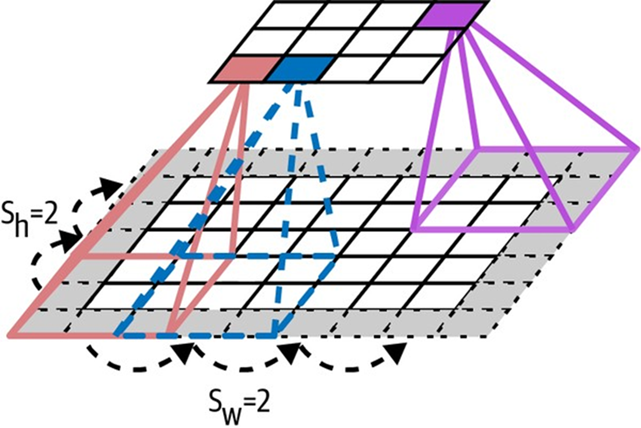
\includegraphics[width=\textwidth,height=0.65\textheight,keepaspectratio]{../machineLearningWeb/Figures/CH14/Hình_14-4}
            \vspace{0.2cm}
            \textit{Hình 14-4: Lớp tích chập với bước nhảy Stride=2}
        \end{column}
    \end{columns}
\end{frame}

\begin{frame}{Bộ lọc (Filters / Kernels)}
    \begin{columns}
        \begin{column}{0.5\textwidth}
            \begin{itemize}
                \item Trọng số của một nơ-ron có thể biểu diễn dưới dạng ma trận kích thước nhỏ, gọi là \textbf{Filter}.
                \item \textbf{Hình 14-5} minh họa hai bộ lọc cổ điển:
                \begin{itemize}
                    \item Bộ lọc dọc (Vertical filter): Nhấn mạnh các đường nét thẳng đứng.
                    \item Bộ lọc ngang (Horizontal filter): Nhấn mạnh các đường nét nằm ngang.
                \end{itemize}
                \item Trong CNN, ta \textit{không tự định nghĩa filter}, mạng nơ-ron sẽ \textbf{tự học} các giá trị bộ lọc tốt nhất cho tác vụ.
            \end{itemize}
        \end{column}
        \begin{column}{0.5\textwidth}
            \centering
            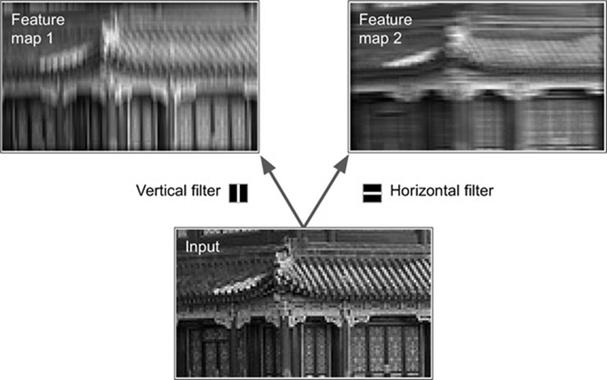
\includegraphics[width=\textwidth,height=0.7\textheight,keepaspectratio]{../machineLearningWeb/Figures/CH14/Hình_14-5}
            \vspace{0.2cm}
            \textit{Hình 14-5: Áp dụng các bộ lọc khác nhau lên ảnh}
        \end{column}
    \end{columns}
\end{frame}

\begin{frame}{Nhiều Bản đồ Đặc trưng (Feature Maps)}
    \begin{columns}
        \begin{column}{0.5\textwidth}
            \begin{itemize}
                \item Trong thực tế, một lớp tích chập sẽ có nhiều bộ lọc (ví dụ: 64 bộ lọc).
                \item Mỗi bộ lọc sinh ra một \textbf{Bản đồ đặc trưng (Feature map)} 2D.
                \item \textbf{Hình 14-6} mô phỏng quá trình đầu vào 3 kênh (RGB) quét qua nhiều bộ lọc để sinh ra một khối dữ liệu 3D đầu ra (Số kênh bằng số bộ lọc).
            \end{itemize}
        \end{column}
        \begin{column}{0.5\textwidth}
            \centering
            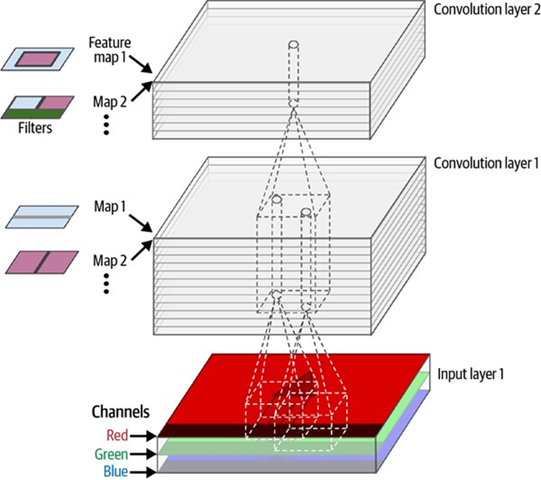
\includegraphics[width=\textwidth,height=0.7\textheight,keepaspectratio]{../machineLearningWeb/Figures/CH14/Hình_14-6}
            \vspace{0.2cm}
            \textit{Hình 14-6: Đầu vào đa kênh và Đầu ra đa kênh}
        \end{column}
    \end{columns}
\end{frame}

\begin{frame}{Padding: "Valid" vs "Same"}
    \begin{columns}
        \begin{column}{0.5\textwidth}
            \begin{itemize}
                \item Keras hỗ trợ 2 tham số phổ biến:
                \item \texttt{padding="valid"}: KHÔNG dùng padding. Bộ lọc có thể vượt ra ngoài biên, làm ảnh bị thu nhỏ lại nhanh chóng (bên phải \textbf{Hình 14-7}).
                \item \texttt{padding="same"}: Có padding. Đảm bảo kích thước ảnh ra bẳng ảnh vào nếu stride=1 (bên trái \textbf{Hình 14-7}).
            \end{itemize}
        \end{column}
        \begin{column}{0.5\textwidth}
            \centering
            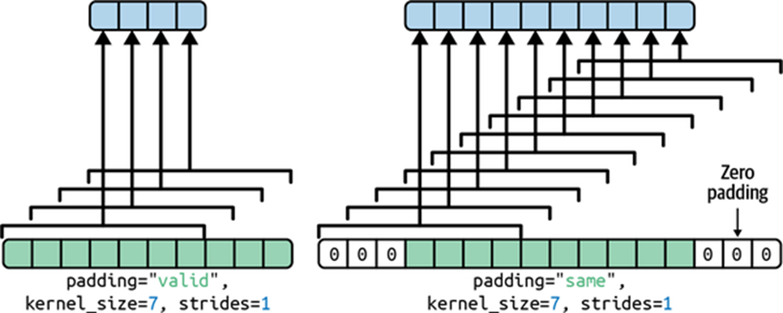
\includegraphics[width=\textwidth,height=0.65\textheight,keepaspectratio]{../machineLearningWeb/Figures/CH14/Hình_14-7}
            \vspace{0.2cm}
            \textit{Hình 14-7: Cài đặt Padding SAME và VALID}
        \end{column}
    \end{columns}
\end{frame}

\begin{frame}[fragile]{Code: Xây dựng Lớp Conv2D trong Keras}
    Để thêm một lớp Tích chập (Convolution) vào mạng:
\begin{lstlisting}[language=Python]
from tensorflow import keras

model = keras.models.Sequential([
    keras.layers.Conv2D(filters=64, kernel_size=7, activation="relu",
                        padding="same", input_shape=[28, 28, 1])
])
\end{lstlisting}
    \begin{itemize}
        \item \texttt{filters=64}: Mạng sẽ tự học 64 bộ lọc khác nhau.
        \item \texttt{kernel\_size=7}: Kích thước bộ lọc là $7\times7$.
        \item Lớp này đòi hỏi rất nhiều phép tính bộ nhớ, nhưng số lượng \textit{tham số (weights)} lại rất ít (do có cơ chế chia sẻ trọng số).
    \end{itemize}
\end{frame}

\begin{frame}{Công thức Tính Kích Thước Đầu Ra (Output Dimension)}
    \begin{itemize}
        \item Kích thước của Bản đồ đặc trưng đầu ra (Feature Map) sau một lớp tích chập được tính bằng công thức:
        \begin{equation*}
            O = \left\lfloor \frac{I - F + 2P}{S} \right\rfloor + 1
        \end{equation*}
        \item Trong đó:
        \begin{itemize}
            \item $O$: Kích thước không gian đầu ra (Output dimension).
            \item $I$: Kích thước không gian đầu vào (Input dimension).
            \item $F$: Kích thước trường tiếp nhận của nơ-ron (Filter size/Receptive field).
            \item $P$: Lượng đệm (Zero Padding) được thêm vào mỗi phía.
            \item $S$: Bước nhảy (Stride).
        \end{itemize}
        \item Nếu padding="same", kích thước đầu ra $O = \lceil I / S \rceil$.
    \end{itemize}
\end{frame}

\begin{frame}{Lớp Gộp Trung Bình \& Gộp Toàn Cục}
    \begin{columns}
        \begin{column}{0.5\textwidth}
            \begin{itemize}
                \item \textbf{Average Pooling (Gộp Trung bình):} Thay vì lấy giá trị max, nó tính trung bình tất cả các giá trị trong trường tiếp nhận. Nó từng phổ biến ở LeNet-5, nhưng nay ít dùng hơn Max Pooling vì Max Pooling bảo toàn đường nét mạnh mẽ hơn.
                \item \textbf{Global Average Pooling (GAP):} Lấy trung bình toàn bộ một Bản đồ đặc trưng (kích thước n x n thu gọn thành 1 con số duy nhất). 
                \item Rất hay dùng ở lớp cuối cùng trước Softmax, giúp giảm lượng tham số khổng lồ (\textbf{Hình 14-10}).
            \end{itemize}
        \end{column}
        \begin{column}{0.5\textwidth}
            \centering
            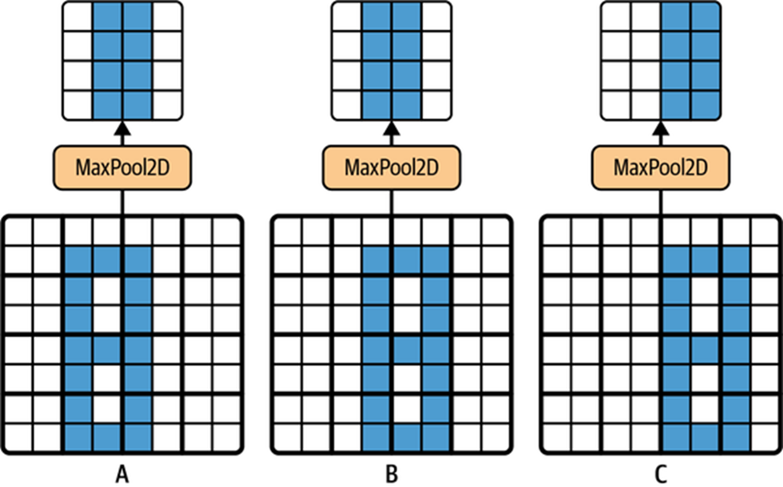
\includegraphics[width=\textwidth,height=0.65\textheight,keepaspectratio]{../machineLearningWeb/Figures/CH14/Hình_14-10}
            \vspace{0.2cm}
            \textit{Hình 14-10: Các phương pháp Pooling khác}
        \end{column}
    \end{columns}
\end{frame}

\begin{frame}{Lớp Gộp (Pooling Layer)}
    \begin{columns}
        \begin{column}{0.5\textwidth}
            \begin{itemize}
                \item Sau vài lớp Tích chập, số kênh tăng rất nhiều (vd: 256, 512). Cần phải giảm không gian (chiều rộng và chiều cao) để tiết kiệm tài nguyên.
                \item \textbf{Lớp Gộp (Pooling Layer)} ra đời để làm giảm khối lượng dữ liệu (Downsampling).
                \item Hình ảnh 14-8 (nếu có) thường mô tả ý tưởng chung của Downsampling.
            \end{itemize}
        \end{column}
        \begin{column}{0.5\textwidth}
            \centering
            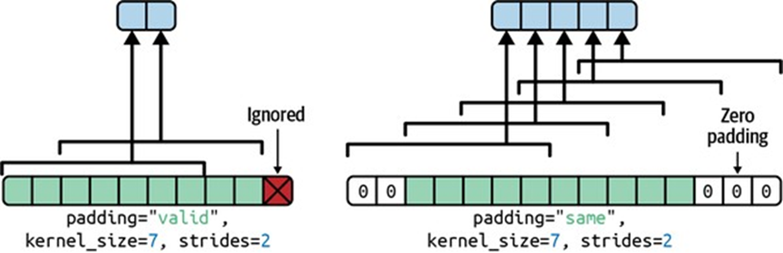
\includegraphics[width=\textwidth,height=0.6\textheight,keepaspectratio]{../machineLearningWeb/Figures/CH14/Hình_14-8}
            \vspace{0.2cm}
            \textit{Hình 14-8: Ý tưởng của Pooling}
        \end{column}
    \end{columns}
\end{frame}

\begin{frame}{Max Pooling (Gộp Cực Đại)}
    \begin{columns}
        \begin{column}{0.5\textwidth}
            \begin{itemize}
                \item Phổ biến nhất là \textbf{Max Pooling}. 
                \item \textbf{Hình 14-9} cho thấy kernel $2\times2$, stride=2.
                \item Quét qua vùng $2\times2$, nó chọn ra phần tử có giá trị lớn nhất (ví dụ: max của [1, 5, 3, 2] là 5).
                \item Lợi ích: Chọn ra các đặc trưng nổi bật nhất, và mang lại tính chất \textbf{bất biến đối với dịch chuyển nhỏ} (Translation Invariance).
            \end{itemize}
        \end{column}
        \begin{column}{0.5\textwidth}
            \centering
            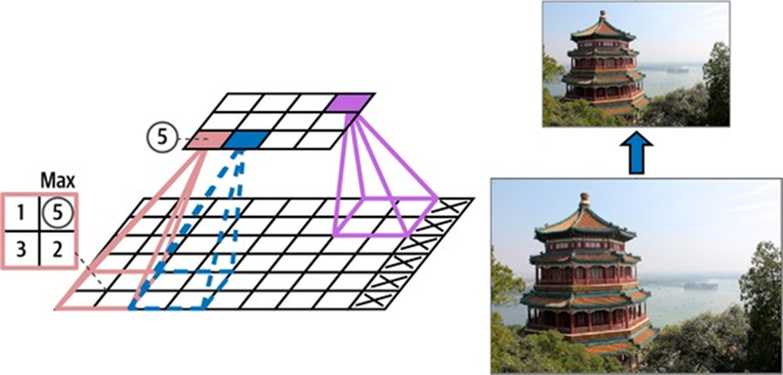
\includegraphics[width=\textwidth,height=0.65\textheight,keepaspectratio]{../machineLearningWeb/Figures/CH14/Hình_14-9}
            \vspace{0.2cm}
            \textit{Hình 14-9: Lớp gộp cực đại (Max Pooling Layer)}
        \end{column}
    \end{columns}
\end{frame}

\begin{frame}{Tính Bất Biến đối với Dịch Chuyển (Translation Invariance)}
    \begin{columns}
        \begin{column}{0.5\textwidth}
            \begin{itemize}
                \item \textbf{Hình 14-11} minh họa: Chữ số C dịch sang phải vài pixel.
                \item Ở các lớp dưới, Max Pooling bảo toàn đường nét chính dù có xê dịch.
                \item Kết quả là vector đặc trưng đầu ra của lớp cuối cùng gần như không đổi. 
                \item Điều này vô cùng có lợi cho phân loại, không cần phải dạy mạng học từng vị trí của con mèo trong ảnh.
            \end{itemize}
        \end{column}
        \begin{column}{0.5\textwidth}
            \centering
            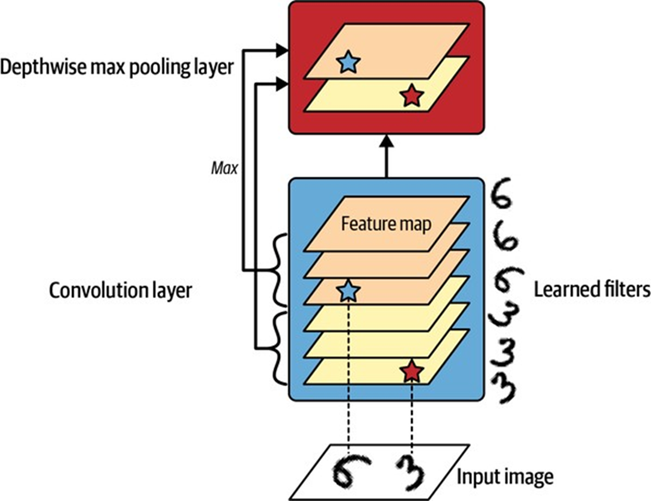
\includegraphics[width=\textwidth,height=0.7\textheight,keepaspectratio]{../machineLearningWeb/Figures/CH14/Hình_14-11}
            \vspace{0.2cm}
            \textit{Hình 14-11: Tính bất biến nhờ Max Pooling}
        \end{column}
    \end{columns}
\end{frame}

\begin{frame}{Tổng hợp Kiến Trúc CNN Tiêu Chuẩn}
    \begin{columns}
        \begin{column}{0.4\textwidth}
            \begin{itemize}
                \item \textbf{Hình 14-12} tổng hợp một quy trình chuẩn:
                \begin{enumerate}
                    \item Cụm (Conv + ReLU + Conv + ReLU + MaxPool). Lặp lại vài lần.
                    \item Ảnh nhỏ dần nhưng Dày lên (nhiều feature maps).
                    \item Lớp Flatten: Duỗi thẳng thành vector 1D.
                    \item Các lớp Dense (Fully Connected) đóng vai trò bộ phân loại.
                    \item Output layer (Softmax).
                \end{enumerate}
            \end{itemize}
        \end{column}
        \begin{column}{0.6\textwidth}
            \centering
            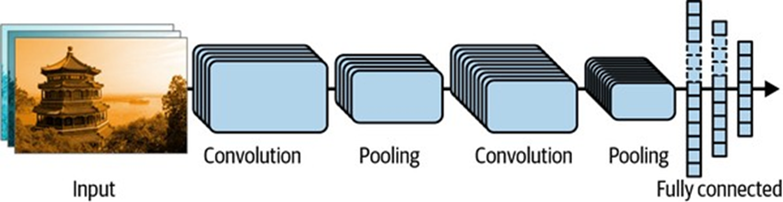
\includegraphics[width=\textwidth,height=0.65\textheight,keepaspectratio]{../machineLearningWeb/Figures/CH14/Hình_14-12}
            \vspace{0.2cm}
            \textit{Hình 14-12: Mạng Nơ-ron Tích chập điển hình}
        \end{column}
    \end{columns}
\end{frame}

\section{3. Kiến trúc CNN Tiêu Biểu (Lịch sử \& Hiện đại)}

\begin{frame}{1. LeNet-5 (1998)}
    \begin{itemize}
        \item Tác giả: Yann LeCun.
        \item Ứng dụng: Nhận diện mã bưu điện viết tay trên phong bì.
        \item Kiến trúc kinh điển đầu tiên kết hợp Convolution và Average Pooling.
        \item Đặt nền móng cho cuộc cách mạng Deep Learning.
    \end{itemize}
\end{frame}

\begin{frame}{2. AlexNet (2012)}
    \begin{itemize}
        \item Chiến thắng vang dội tại cuộc thi ImageNet ILSVRC 2012.
        \item Kiến trúc sâu hơn LeNet-5. Lần đầu tiên sử dụng hàm kích hoạt ReLU, giúp mạng học cực nhanh.
        \item Lần đầu tiên sử dụng kĩ thuật chống quá khớp đột phá là \textbf{Dropout}.
        \item Chạy trên 2 GPU NVIDIA vì GPU ngày đó không đủ RAM để chứa cả mô hình.
    \end{itemize}
\end{frame}

\begin{frame}{Tăng cường Dữ liệu (Data Augmentation)}
    \begin{columns}
        \begin{column}{0.5\textwidth}
            \begin{itemize}
                \item AlexNet nổi tiếng với việc tạo ra dữ liệu giả khổng lồ từ dữ liệu thật.
                \item \textbf{Hình 14-13} minh họa quá trình: Từ 1 ảnh gốc con ếch, tạo ra hàng chục ảnh đã bị lật ngang, lật dọc, dịch chuyển, xoay, thay đổi màu sắc.
                \item Việc này giúp mô hình chống overfit và ép nó học các tính chất bất biến phức tạp hơn.
            \end{itemize}
        \end{column}
        \begin{column}{0.5\textwidth}
            \centering
            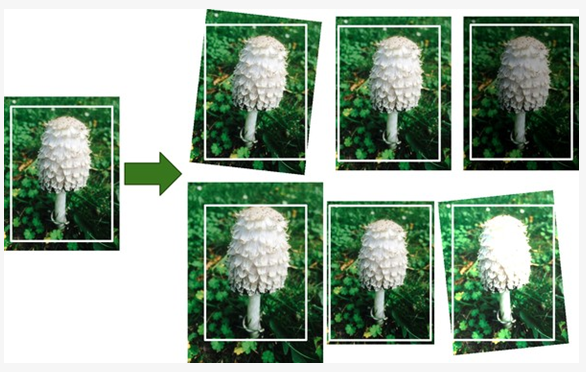
\includegraphics[width=\textwidth,height=0.6\textheight,keepaspectratio]{../machineLearningWeb/Figures/CH14/Hình_14-13}
            \vspace{0.2cm}
            \textit{Hình 14-13: Tăng cường dữ liệu (Data Augmentation)}
        \end{column}
    \end{columns}
\end{frame}

\begin{frame}{3. GoogLeNet (2014) và Mô đun Inception}
    \begin{columns}
        \begin{column}{0.4\textwidth}
            \begin{itemize}
                \item Lỗi 10\% trên ImageNet xuống còn <7\%.
                \item Bí quyết là các mô-đun \textbf{Inception} (\textbf{Hình 14-14}).
                \item Thay vì hỏi: "Nên dùng Kernel 1x1, 3x3 hay 5x5?", GoogLeNet \textbf{dùng TẤT CẢ} cùng lúc trong 1 mô-đun.
                \item Đặc biệt sử dụng nhiều Conv 1x1 để "bóp" số lượng kênh, giảm khối lượng tính toán.
            \end{itemize}
        \end{column}
        \begin{column}{0.6\textwidth}
            \centering
            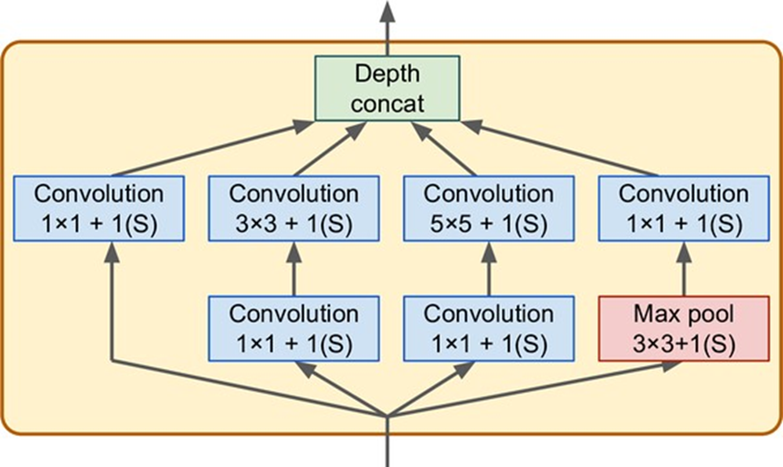
\includegraphics[width=\textwidth,height=0.7\textheight,keepaspectratio]{../machineLearningWeb/Figures/CH14/Hình_14-14}
            \vspace{0.2cm}
            \textit{Hình 14-14: Kiến trúc một mô-đun Inception}
        \end{column}
    \end{columns}
\end{frame}

\begin{frame}{Mạng GoogLeNet Hoàn Chỉnh}
    \begin{center}
        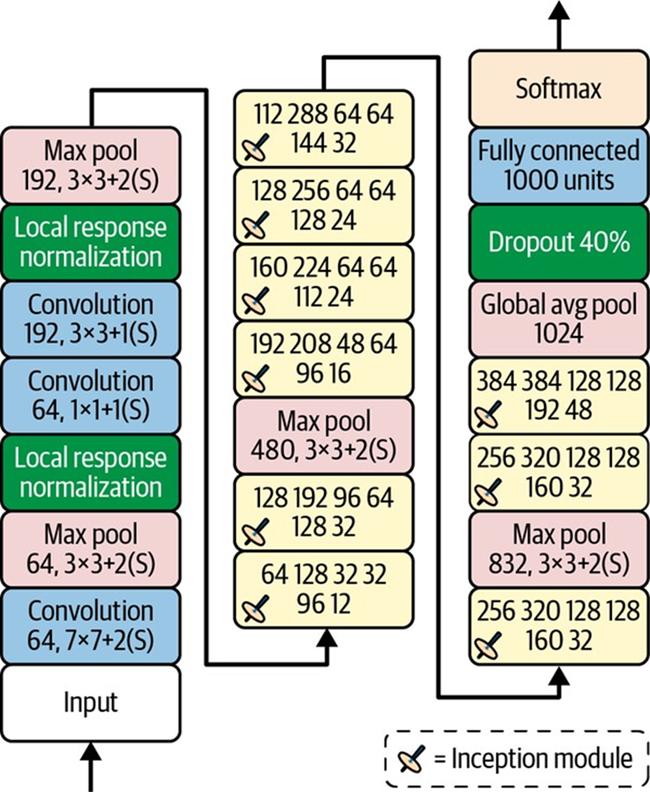
\includegraphics[width=0.9\textwidth,height=0.7\textheight,keepaspectratio]{../machineLearningWeb/Figures/CH14/Hình_14-15}
        
        \vspace{0.2cm}
        \textit{Hình 14-15: Toàn cảnh Kiến trúc GoogLeNet sâu thẳm}
    \end{center}
\end{frame}

\begin{frame}{4. ResNet (2015) - Residual Networks}
    \begin{columns}
        \begin{column}{0.5\textwidth}
            \begin{itemize}
                \item Khi mạng quá sâu (hơn 30 lớp), lỗi huấn luyện lại tăng do Gradient suy thoái.
                \item ResNet giải quyết bằng \textbf{Kết nối tắt (Skip Connections)}.
                \item Thay vì học trực tiếp một hàm $H(x)$, ResNet học \textbf{phần dư} $F(x) = H(x) - x$. 
                \item \textbf{Hình 14-16} minh họa khối dư (Residual block).
            \end{itemize}
        \end{column}
        \begin{column}{0.5\textwidth}
            \centering
            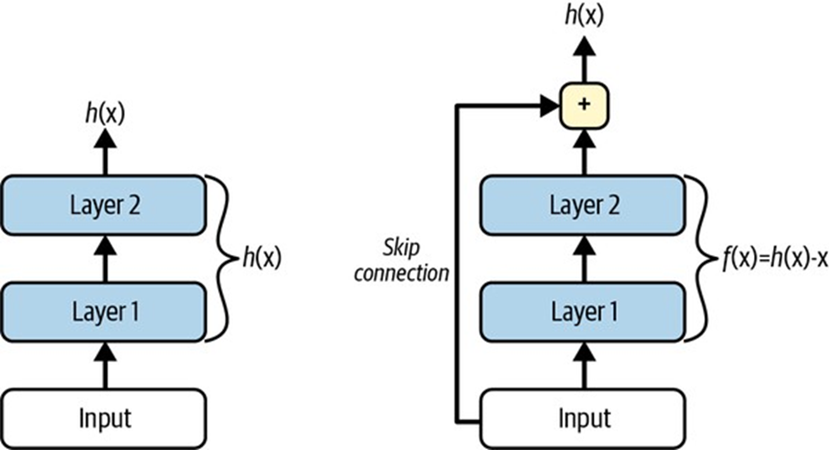
\includegraphics[width=\textwidth,height=0.6\textheight,keepaspectratio]{../machineLearningWeb/Figures/CH14/Hình_14-16}
            \vspace{0.2cm}
            \textit{Hình 14-16: Khối Residual Learning cơ bản}
        \end{column}
    \end{columns}
\end{frame}

\begin{frame}{Cơ chế Hoạt động của Skip Connection}
    \begin{columns}
        \begin{column}{0.5\textwidth}
            \begin{itemize}
                \item \textbf{Hình 14-17} so sánh Mạng thường (Regular Network) và Mạng Dư thừa (Residual Network).
                \item Lợi ích: Dòng chảy gradient truyền trực tiếp qua nét liền $x$, không bị suy giảm.
                \item Cho phép mạng sâu tới 152 lớp (ResNet-152) mà huấn luyện vẫn hội tụ rất nhanh.
            \end{itemize}
        \end{column}
        \begin{column}{0.5\textwidth}
            \centering
            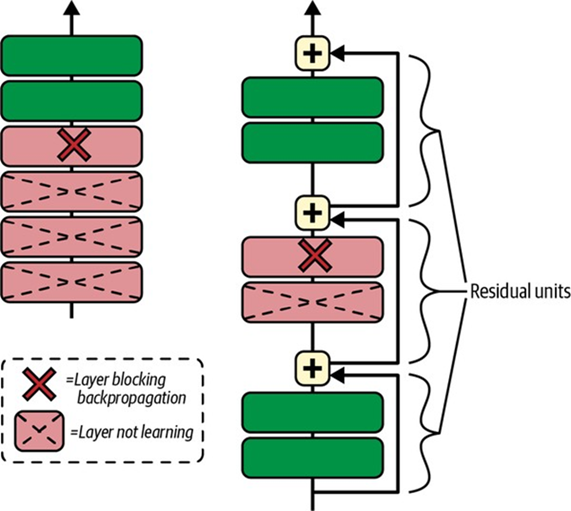
\includegraphics[width=\textwidth,height=0.65\textheight,keepaspectratio]{../machineLearningWeb/Figures/CH14/Hình_14-17}
            \vspace{0.2cm}
            \textit{Hình 14-17: Mạng lưới sâu với kết nối bỏ qua}
        \end{column}
    \end{columns}
\end{frame}

\begin{frame}{Toàn Cảnh Kiến Trúc ResNet}
    \begin{columns}
        \begin{column}{0.35\textwidth}
            \begin{itemize}
                \item \textbf{Hình 14-18}: Mạng ResNet xếp chồng hàng chục khối RU liên tục.
                \item Ở các điểm mốc (đường nét đứt), số kênh nhân đôi, bản đồ đặc trưng thu nhỏ lại một nửa (thông qua Stride=2).
            \end{itemize}
        \end{column}
        \begin{column}{0.65\textwidth}
            \centering
            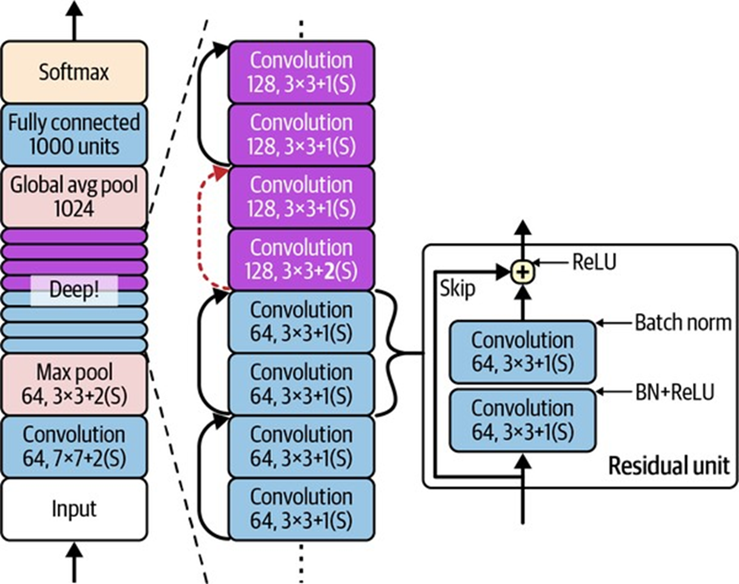
\includegraphics[width=\textwidth,height=0.8\textheight,keepaspectratio]{../machineLearningWeb/Figures/CH14/Hình_14-18}
            \vspace{0.2cm}
            \textit{Hình 14-18: Kiến trúc tổng thể ResNet}
        \end{column}
    \end{columns}
\end{frame}

\begin{frame}[fragile]{Code: Xây dựng Khối Residual (ResNet Block)}
\begin{lstlisting}[language=Python]
class ResidualUnit(keras.layers.Layer):
    def __init__(self, filters, strides=1, activation="relu", **kwargs):
        super().__init__(**kwargs)
        self.activation = keras.activations.get(activation)
        self.main_layers = [
            keras.layers.Conv2D(filters, 3, strides=strides, padding="same", use_bias=False),
            keras.layers.BatchNormalization(),
            self.activation,
            keras.layers.Conv2D(filters, 3, strides=1, padding="same", use_bias=False),
            keras.layers.BatchNormalization()]
        self.skip_layers = []
        if strides > 1:
            self.skip_layers = [
                keras.layers.Conv2D(filters, 1, strides=strides, padding="same", use_bias=False),
                keras.layers.BatchNormalization()]

    def call(self, inputs):
        Z = inputs
        for layer in self.main_layers: Z = layer(Z)
        skip_Z = inputs
        for layer in self.skip_layers: skip_Z = layer(skip_Z)
        return self.activation(Z + skip_Z)
\end{lstlisting}
\end{frame}

\begin{frame}{Xử lý Kích thước Kênh qua Skip Connection}
    \begin{columns}
        \begin{column}{0.5\textwidth}
            \begin{itemize}
                \item Khi thay đổi số lượng bản đồ đặc trưng, ta không thể cộng trực tiếp $F(x) + x$ (Vì khác kích thước ma trận).
                \item Giải pháp: Thêm một lớp \textbf{Conv 1x1 (stride=2)} vào đường chéo (Skip connection) để đồng bộ số lượng bộ lọc.
                \item \textbf{Hình 14-19} mô phỏng kĩ thuật này.
            \end{itemize}
        \end{column}
        \begin{column}{0.5\textwidth}
            \centering
            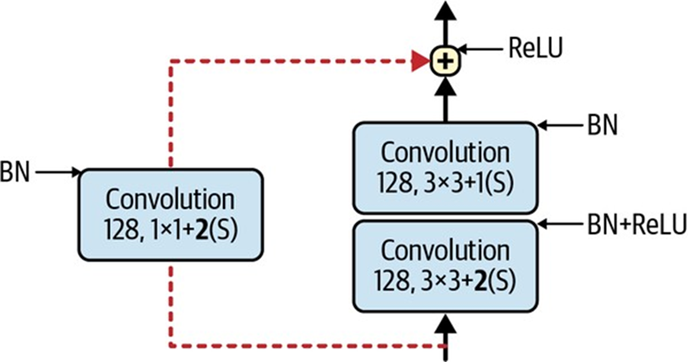
\includegraphics[width=\textwidth,height=0.6\textheight,keepaspectratio]{../machineLearningWeb/Figures/CH14/Hình_14-19}
            \vspace{0.2cm}
            \textit{Hình 14-19: Khối thay đổi kích thước}
        \end{column}
    \end{columns}
\end{frame}

\begin{frame}{5. Xception (2016)}
    \begin{columns}
        \begin{column}{0.5\textwidth}
            \begin{itemize}
                \item Tác giả: Francois Chollet (Cha đẻ của Keras).
                \item Tên gọi Xception = "Extreme Inception".
                \item Tách biệt hoàn toàn Không gian (Spatial) và Kênh (Cross-Channel).
                \item Sử dụng \textbf{Depthwise Separable Convolution} (\textbf{Hình 14-20}) và (\textbf{Hình 14-21}).
                \item Ưu điểm: Tốn ít bộ nhớ và tham số hơn Inception rất nhiều nhưng hiệu năng tốt hơn.
            \end{itemize}
        \end{column}
        \begin{column}{0.5\textwidth}
            \centering
            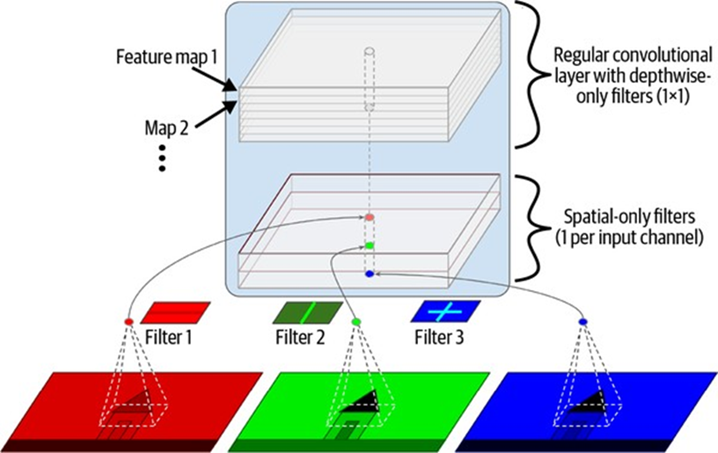
\includegraphics[width=\textwidth,height=0.45\textheight,keepaspectratio]{../machineLearningWeb/Figures/CH14/Hình_14-20}
            
            \vspace{0.1cm}
            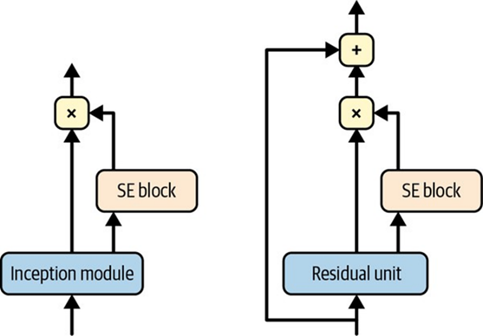
\includegraphics[width=\textwidth,height=0.35\textheight,keepaspectratio]{../machineLearningWeb/Figures/CH14/Hình_14-21}
            \vspace{0.2cm}
            \textit{Hình 14-20 \& 14-21: Khái niệm Depthwise Separable Conv}
        \end{column}
    \end{columns}
\end{frame}

\begin{frame}{6. SENet (2017) - Squeeze-and-Excitation}
    \begin{columns}
        \begin{column}{0.5\textwidth}
            \begin{itemize}
                \item Đạt giải nhất ImageNet 2017.
                \item Nâng cấp mọi mạng hiện có bằng việc gắn thêm \textbf{Khối SE} (\textbf{Hình 14-22}).
                \item Khối SE tự động học để "đánh trọng số" mức độ quan trọng cho các Bản đồ đặc trưng (kênh). (Vd: Nếu thấy cái mũi, lập tức tăng cường các bộ lọc của con mắt/miệng để tìm khuôn mặt).
            \end{itemize}
        \end{column}
        \begin{column}{0.5\textwidth}
            \centering
            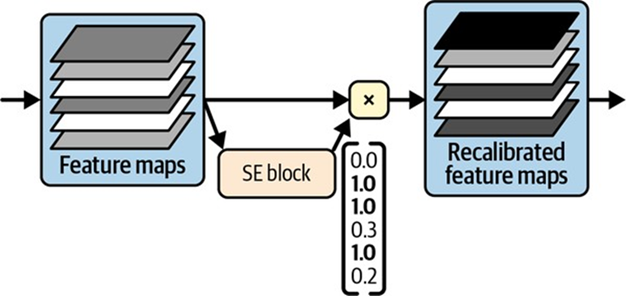
\includegraphics[width=\textwidth,height=0.7\textheight,keepaspectratio]{../machineLearningWeb/Figures/CH14/Hình_14-22}
            \vspace{0.2cm}
            \textit{Hình 14-22: Khối SE (Squeeze-and-Excitation)}
        \end{column}
    \end{columns}
\end{frame}

\begin{frame}{Mô-đun SE-Inception}
    \begin{center}
        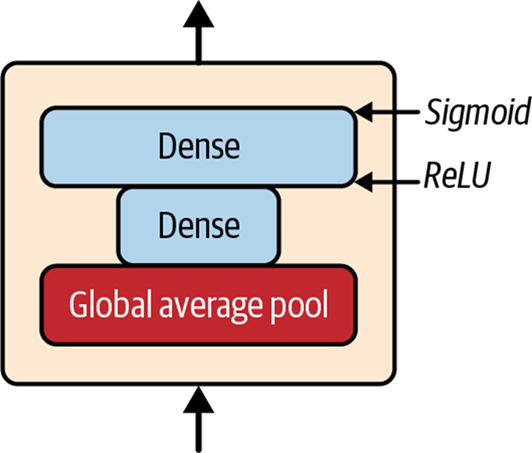
\includegraphics[width=0.85\textwidth,height=0.7\textheight,keepaspectratio]{../machineLearningWeb/Figures/CH14/Hình_14-23}
        
        \vspace{0.2cm}
        \textit{Hình 14-23: Tích hợp SE block vào mô-đun Inception}
    \end{center}
\end{frame}

\begin{frame}[fragile]{Sử dụng Mô Hình Sẵn Có (Pretrained) trong Keras}
    Trong thực tế, hiếm khi chúng ta đào tạo mạng ResNet từ đầu (Scratch). Keras cung cấp sẵn \textbf{Transfer Learning}:
\begin{lstlisting}[language=Python]
from tensorflow.keras.applications import resnet50

# Load model voi trong so (weights) da huan luyen tren ImageNet
model = resnet50.ResNet50(weights="imagenet")

# Xu ly anh ve dung kich thuoc yeu cau
X_resized = tf.image.resize(images, [224, 224])
X_input = resnet50.preprocess_input(X_resized)

Y_proba = model.predict(X_input)
\end{lstlisting}
    \begin{itemize}
        \item Mạng tải xuống đã có khả năng nhận dạng 1000 lớp đồ vật khác nhau vô cùng chính xác.
    \end{itemize}
\end{frame}

\section{4. Định Vị Đối Tượng (Object Localization)}

\begin{frame}{Bài toán Phân loại và Định vị}
    \begin{itemize}
        \item Cùng với việc \textbf{Phân loại (Classification)}: "Đó là hoa gì?", máy tính có thể \textbf{Định vị (Localization)}: "Hoa đó nằm ở đâu trong ảnh?".
        \item Đầu ra của mạng bây giờ có thêm 4 giá trị số thực (Regression) đại diện cho \textbf{Bounding Box (Khung chứa)}:
        \begin{itemize}
            \item Tọa độ tâm: $x, y$
            \item Kích thước khung: $height, width$
        \end{itemize}
        \item Hàm Loss: \textbf{MSE} (Sai số toàn phương) dùng cho Bounding Box, cộng gộp với \textbf{Cross-Entropy} của bộ phân loại.
    \end{itemize}
\end{frame}

\begin{frame}{Đo lường Khung Chứa: IoU (Intersection over Union)}
    \begin{columns}
        \begin{column}{0.5\textwidth}
            \begin{itemize}
                \item Làm thế nào để biết hệ thống dự đoán $x,y,w,h$ có tốt hay không?
                \item Ta dùng chỉ số \textbf{IoU}.
                \item Tính bằng: $Diện tích \ Giao \ / \ Diện tích \ Hợp$
                \item \textbf{Hình 14-24} giải thích IoU. Nếu hộp đỏ và hộp xanh lá đè lên nhau hoàn hảo, IoU = 1.0. Nếu lệnh hẳn, IoU = 0.
            \end{itemize}
        \end{column}
        \begin{column}{0.5\textwidth}
            \centering
            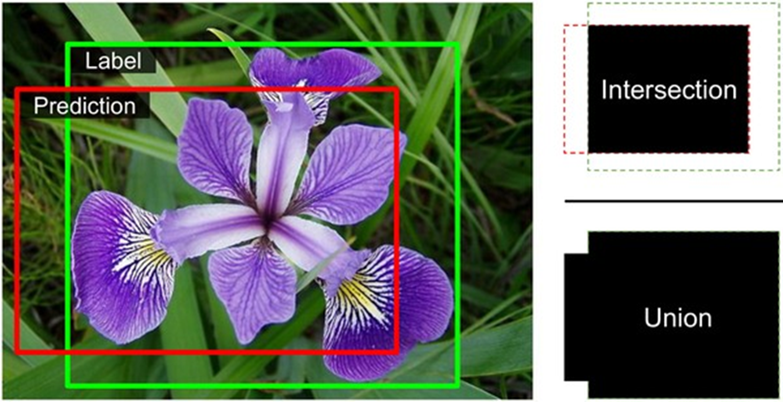
\includegraphics[width=\textwidth,height=0.65\textheight,keepaspectratio]{../machineLearningWeb/Figures/CH14/Hình_14-24}
            \vspace{0.2cm}
            \textit{Hình 14-24: Đánh giá bằng IoU}
        \end{column}
    \end{columns}
\end{frame}

\begin{frame}{Thuật toán Non-Max Suppression}
    \begin{itemize}
        \item Trong phát hiện đối tượng, hệ thống có thể tạo ra \textbf{rất nhiều Hộp Bounding Box} đè lên nhau cho cùng một đối tượng (do trượt cửa sổ).
        \item Để loại bỏ hộp thừa, thuật toán \textbf{Non-Max Suppression (NMS)} được sử dụng:
        \begin{enumerate}
            \item Loại bỏ tất cả hộp có xác suất chứa đối tượng (Objectness score) dưới một ngưỡng nhất định (ví dụ: < 0.5).
            \item Chọn hộp có xác suất cao nhất.
            \item Tính IoU của hộp này với các hộp còn lại.
            \item Loại bỏ (Suppress) tất cả các hộp khác có IoU $\ge$ 0.6 so với hộp cao nhất.
            \item Lặp lại bước 2 cho đến khi không còn hộp nào chưa xét.
        \end{enumerate}
    \end{itemize}
\end{frame}

\begin{frame}{Mean Average Precision (mAP)}
    \begin{itemize}
        \item Làm thế nào để đánh giá toàn diện mô hình Object Detection?
        \item Một Bounding Box được xem là "Đúng" (True Positive) nếu: 
            \begin{enumerate}
                \item Dự đoán đúng Lớp.
                \item IoU $\ge$ một ngưỡng (vd 0.5 hoặc 0.75).
            \end{enumerate}
        \item Từ đó ta vẽ đường cong Precision/Recall. Diện tích dưới đường cong là \textbf{Average Precision (AP)} của 1 lớp.
        \item Lấy trung bình AP của TẤT CẢ các lớp, ta được \textbf{mAP (mean Average Precision)}.
    \end{itemize}
\end{frame}

\section{5. Phát hiện Đối Tượng (Object Detection)}

\begin{frame}{Bài toán Phát Hiện Đối Tượng}
    \begin{itemize}
        \item Định vị (Localization) chỉ tìm \textbf{một} đối tượng chính.
        \item Phát hiện (Detection) là tìm \textbf{nhiều} đối tượng thuộc nhiều lớp trong cùng một ảnh.
        \item Cách ngây thơ nhất là \textbf{Sliding Window (Cửa sổ trượt)}: Cắt ảnh thành nhiều hình vuông nhỏ và chạy bộ phân loại trên từng hình nhỏ đó. Rất tốn kém!
    \end{itemize}
\end{frame}

\begin{frame}{Biến CNN thành FCN (Fully Convolutional Network)}
    \begin{columns}
        \begin{column}{0.4\textwidth}
            \begin{itemize}
                \item \textbf{Hình 14-26}: Thay vì dùng lớp Dense ở cuối, ta có thể thay thế nó bằng lớp Tích chập $1\times1$.
                \item Mạng bây giờ không có ràng buộc về kích thước đầu vào nữa (vì không có lớp duỗi Flatten).
                \item Nó trở thành mạng tích chập hoàn toàn (FCN).
            \end{itemize}
        \end{column}
        \begin{column}{0.6\textwidth}
            \centering
            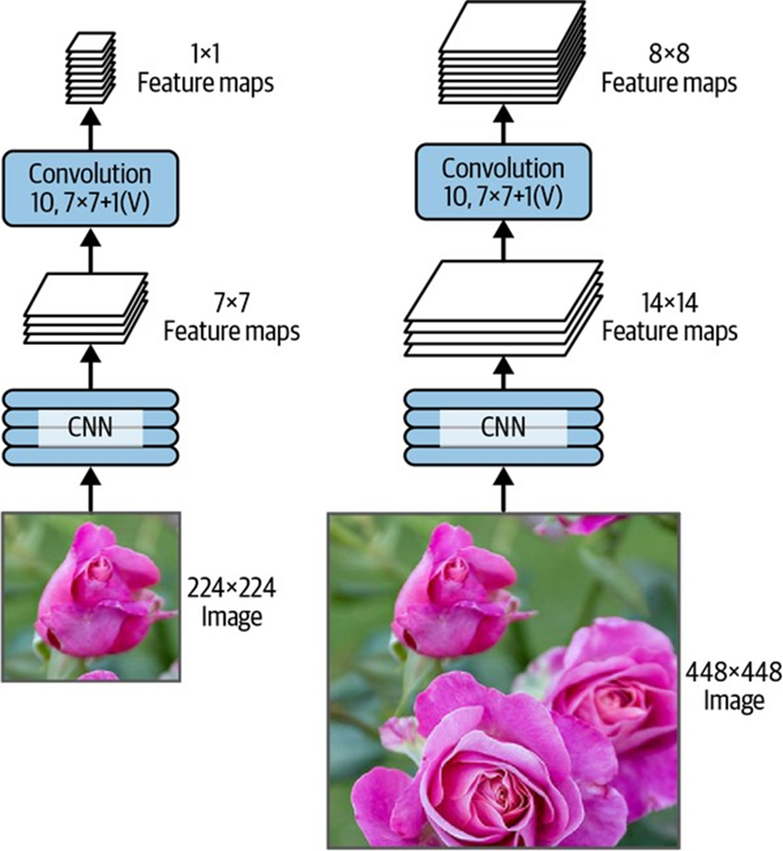
\includegraphics[width=\textwidth,height=0.7\textheight,keepaspectratio]{../machineLearningWeb/Figures/CH14/Hình_14-26}
            \vspace{0.2cm}
            \textit{Hình 14-26: Chuyển đổi CNN thành FCN}
        \end{column}
    \end{columns}
\end{frame}

\begin{frame}{Giải thuật Yolo (You Only Look Once)}
    \begin{columns}
        \begin{column}{0.45\textwidth}
            \begin{itemize}
                \item YOLO (2015) sử dụng FCN để tạo ra một cuộc cách mạng.
                \item Nó chia ảnh thành một lưới (Grid) kích thước $5\times7$.
                \item Mỗi ô lưới dự đoán Bounding Box cho đối tượng nằm ở tâm của ô lưới đó (\textbf{Hình 14-25}).
                \item YOLO chạy siêu nhanh, thời gian thực (Real-time).
            \end{itemize}
        \end{column}
        \begin{column}{0.55\textwidth}
            \centering
            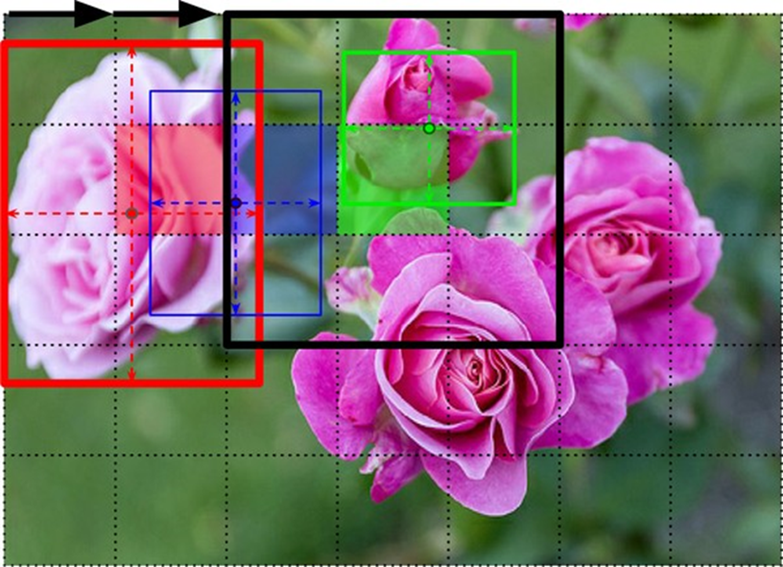
\includegraphics[width=\textwidth,height=0.7\textheight,keepaspectratio]{../machineLearningWeb/Figures/CH14/Hình_14-25}
            \vspace{0.2cm}
            \textit{Hình 14-25: Phát hiện đối tượng theo dạng lưới lưới (Grid)}
        \end{column}
    \end{columns}
\end{frame}

\section{6. Phân đoạn Ngữ nghĩa (Semantic Segmentation)}

\begin{frame}{Bài toán Phân Đoạn Ngữ Nghĩa}
    \begin{columns}
        \begin{column}{0.5\textwidth}
            \begin{itemize}
                \item Không chỉ là khung chứa, hệ thống phải gán \textbf{mỗi pixel} một nhãn cụ thể.
                \item \textbf{Hình 14-27} cho thấy chiếc xe đạp, người, đường phố, tất cả đều được tô màu chính xác đến từng đường viền.
                \item Khó khăn: Qua các lớp Max Pooling, ảnh bị thu nhỏ lại và mất chi tiết viền (Edge details).
            \end{itemize}
        \end{column}
        \begin{column}{0.5\textwidth}
            \centering
            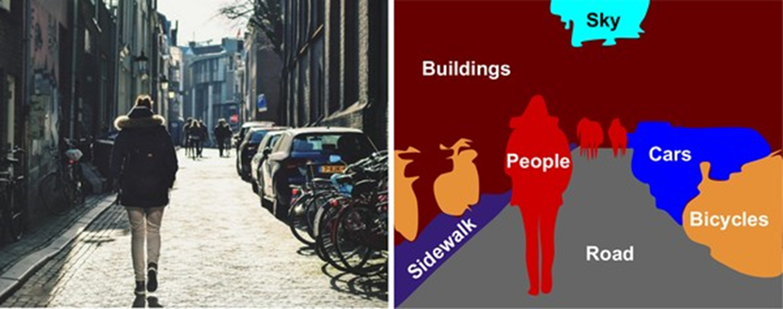
\includegraphics[width=\textwidth,height=0.7\textheight,keepaspectratio]{../machineLearningWeb/Figures/CH14/Hình_14-27}
            \vspace{0.2cm}
            \textit{Hình 14-27: Phân đoạn ngữ nghĩa chi tiết}
        \end{column}
    \end{columns}
\end{frame}

\begin{frame}{Kĩ thuật Tích chập ngược (Transposed Convolution)}
    \begin{columns}
        \begin{column}{0.5\textwidth}
            \begin{itemize}
                \item Để phóng to bức ảnh trở lại kích thước gốc, ta sử dụng \textbf{Tích chập ngược (Up-Sampling)}.
                \item \textbf{Hình 14-28} và \textbf{14-29} mô tả việc chèn thêm các số 0 vào giữa ma trận rồi nhân tích chập để mạng tự học cách nội suy phóng to hình ảnh.
                \item Các mạng như U-Net kết hợp thêm Skip Connection để lấy chi tiết viền từ các lớp ban đầu ghép vào.
            \end{itemize}
        \end{column}
        \begin{column}{0.5\textwidth}
            \centering
            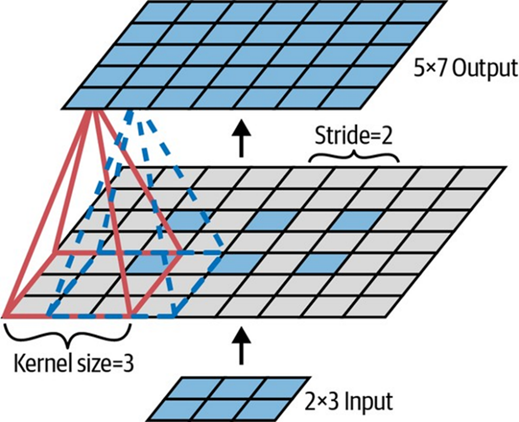
\includegraphics[width=\textwidth,height=0.45\textheight,keepaspectratio]{../machineLearningWeb/Figures/CH14/Hình_14-28}
            
            \vspace{0.1cm}
            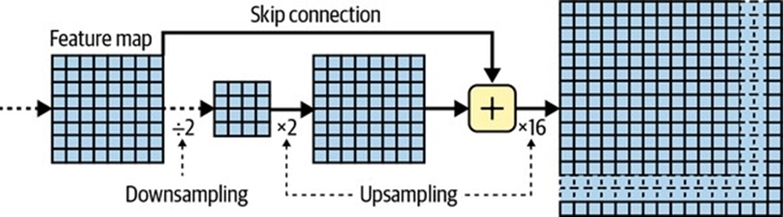
\includegraphics[width=\textwidth,height=0.35\textheight,keepaspectratio]{../machineLearningWeb/Figures/CH14/Hình_14-29}
            \vspace{0.2cm}
            \textit{Hình 14-28, 14-29: Phép tích chập ngược (Up-sampling)}
        \end{column}
    \end{columns}
\end{frame}

\section{Tổng Kết}

\begin{frame}{Tổng Kết Chương 14}
    \begin{itemize}
        \item \textbf{CNN:} Phá vỡ giới hạn của Mạng truyền thẳng bằng cách áp dụng Tích chập cục bộ (Local Receptive Fields) kết hợp Chia sẻ trọng số (Weight sharing).
        \item Các khối cốt lõi: Convolutional Layer, Padding, Strides, Pooling (Max/Avg).
        \item \textbf{Lịch sử Kiến trúc:} Từ LeNet (1998) đơn giản, tới đột phá ReLU/Dropout của AlexNet, mô đun Inception tối ưu của GoogLeNet, cấu trúc Skip Connection vượt rào độ sâu của ResNet, và SENet.
        \item \textbf{Thị giác nâng cao:} Tái cấu trúc thành Mạng Fully Convolutional Networks cho phép chạy YOLO (Phát hiện đối tượng) và U-Net (Phân đoạn ngữ nghĩa).
    \end{itemize}
\end{frame}

\end{document}
